\documentclass{article}
\usepackage{clrscode}
\usepackage{amsmath}
\usepackage{amssymb}
\usepackage{latexsym}
\usepackage{indentfirst}
\usepackage{graphicx}

\setlength{\parindent}{2em}
\begin{document}
\title{Overview: A 3D Surface Tracking Algorithm}
\author{Yao Ming}
\date{\today}
\maketitle
\newpage


\section{Introduction}

This algorithm constructs a surface model from edge voxels. A voxel is
identified as being on the surface if its second derivative is negative and
changes sign for neighbors in the gradient direction. By this definition, there
can only exist one layer of surface voxels, and the tracking algorithm is simply
a breadth-first search. Moreover, the definition of surface voxels is not
sensitive to gradient directions, thus this approach is robust against
noise. The test results on real data are also reported.
Section 2 discusses the surface voxel identification method. Section 3
introduces the surface tracking algorithm.

\section{Surface Identification}
The section presents a 3D surface identification method based on the Laplacian
of Gaussian Filter, which means the condition for an edge voxel being on a
surface is that the second derivative is negative and changes sign for neighbors
in the gradient direction. With this approach, we have to find the
zero-crossings of the second derivative.
\subsection{Surface Points in Continuous Space}
Suppose there is a step intensity change across an object surface. Let $I(x, y,
z)$ be the intensity function, $(x, y, z)\in  R^3$ , where $R$ is the set of real
numbers. Without loss of generality, suppose the intensity change occurs at the
origin and in the $x$ direction. It will be shown in the following that a
zero-crossing occurs at the origin; thus the origin is the desired surface
point.\par
For a bright object surrounded by a darker background, the intensity
around the surface can be modeled as a one-dimensional step change, $I(x, y,
z)=c(\pi / 2 - \arctan (kx))$ for a sufficiently large constant $k > 0$. The constant $c$
describes the magnitude change and $k$ describes the intensity change rate.\par
To use the Laplacian of Gaussian Filter, we use the smoothing filter $G(x,y,z)$,
a Gaussian filter with variance $\sigma$. Let $w(x,y,z)$ be the secon derivative
in the x-direction of the smoothed function $I(x,y,z)$,
\begin{equation}
  w(x,y,z) = \frac {\partial ^2}{\partial x^2}[G(x,y,z)*I(x,y,z)],
\end{equation}
that is,
\begin{equation}
  w(x) = \frac {1}{\sqrt{2\pi}\sigma} \int_{-\infty}^{\infty} e^{-x'^{2} /
    2\sigma^2} \frac {2ck^3(x-x')}{(1+k^2(x-x')^2)^2} dx',
\end{equation}
which is a function of x. At $x=0$,$w(0)=0$ and
\begin{equation}
  w'(0) = \frac {2ck^3}{\sqrt{2\pi}\sigma^3}\int _{-\infty}^{\infty} \frac {x'^2
    e^{-x'^{2} /2\sigma^2}}{1+k^2x'^2}dx' >0
\end{equation}
Hence $w(x)$ is monotonically increasing in the neighborhood of $x=0$. In other
words, $w(x)$ changes sign from negative to positive as it crosses zero at
$x=0$. $x=0$ is therefore called a zero-crossing.\par
Let $v = (x,y,z) \in R^3$ and $l$ be a directed line at $v$ pointing outside of the
surface. Writing the above equations in terms of $v$ and $l$, if $v$ is on the
surface, it must satisfy the following conditions:
\begin{equation*}
  w(v) = 0
\end{equation*}
\begin{equation}
    w(v-\delta l) < 0
\end{equation}
\begin{equation*}
    w(v+\delta l) > 0.
\end{equation*}\par
Besides, it's worthwhile to point out that, obviously, the location of
zero-crossings is not sensitive to the direction of the second derivative of an
intensity change. So it's desirable to take the second derivative in a direction
that has a maximum rate of change. Because of the fact that the gradient
direction is the one in which the second derivative of the intensity function
has the maximum change rate, it is a good choice to use the direction $g$, the
gradient direction at $v$, as direction $l$ in equation (4). Then, equation (1)
becomes like this:
\begin{equation}
  w(v) = G_g''(v) * I(v),
\end{equation}
and equation (4) would be like this:
\begin{equation*}
  w(v) = 0
\end{equation*}
\begin{equation}
    w(v-\delta g) < 0
\end{equation}
\begin{equation*}
    w(v+\delta g) > 0.
\end{equation*}  
\subsection{Surface Voxels in Discrete Space}
In discrete space, we would first introduce the concept of the positive layer
and the negative layer of voxels, and then define surface voxels in a discrete
space.\par
Let $I(v) \in N, N = \{0,1,2,...\}$ be an intensity function defined on a discrete
domain, $v=(x,y,z) \in Z^3,Z = \{0,\pm 1,\pm 2,...\}$. For simplicity, $v$ is called
a voxel. Let $G''_g(x, y, z)$ be a finite scale discrete Gaussian filter,
resulting from sampling $G''_g$ in (5) in a finite interval
$(-3\sigma,3\sigma)$, and let $w(x, y, z)$ be the discrete convolution of
$G''_g(x,y,z)$ with $I(x, y, z)$,
\begin{equation}
  w(x,y,z) = G''_g(x,y,z)*I(x,y,z).
\end{equation}
If $v=(x,y,z)$ is a surface voxel, $w(x,y,z)=0.$\par
In discrete space, not many voxels have $w(x,y,z)=0.$ Condition (6) however,
implies that for a bright object surrounded by a darker background and for those
voxels close to a surface, $w(x, y, z)$ is negative inside the object and
positive outside. There can only exist one layer of voxels on which $w(x, y, z)$
is negative and changes sign for neighbors in the gradient direction. This layer
is called the negative layer. Similarly, there exists exactly one positive layer
of voxels. It is possible to define either the negative layer or the positive
layer as the surface. Since the negative layer is part of the object, the
surface is defined as the negative layer of voxels. Zero-crossing voxels can be
treated as either positive or negative and are also included in the surface
set. The first condition of (6) therefore becomes $w(x, y, z) \leq 0$.\par
As another two conditions in (6), we have to test every possible nonzero situation of
the gradient of $I(v)$ at $v$ and get the corresponding conditons in discrete
space. \par
To summarize, for a bright object surrounded by a darker background, if $v(x, y,
z)$ is a surface voxel, it must simultaneously satisfy the following
inequalities:
\begin{equation*}
  w(x,y,z) \leq 0,
\end{equation*}
\begin{equation}
  w(x+1,y,z)w(x-1,y,z)<0, if\nabla_x \neq 0,
\end{equation}
\begin{equation*}
  w(x,y+1,z)w(x,y-1,z)<0, if\nabla_y \neq 0,
\end{equation*}
\begin{equation*}
  w(x,y,z+1)w(x,y,z-1)<0, if\nabla_z \neq 0,
\end{equation*}\par
The inequalities (8) is the condition to identify surface voxels in a discrete
space. Obviously, there is only one layer of voxels that will satisfy the
condition. This makes subsequent surface tracking much easier.
\section{The Surface Tracking Algorithm}
In this section, we can discuss the tracking algorithms based on the definition
of the surface voxel. This algorithms extracts a single layer of surface using
inequalities (8) and converts surface voxels to graphical primitives to
construct a surface model. We would introduce the definition of graphics
primitives first, which is based on the extended cuberille model.

\subsection{The Extended Cuberille Model}

\centerline{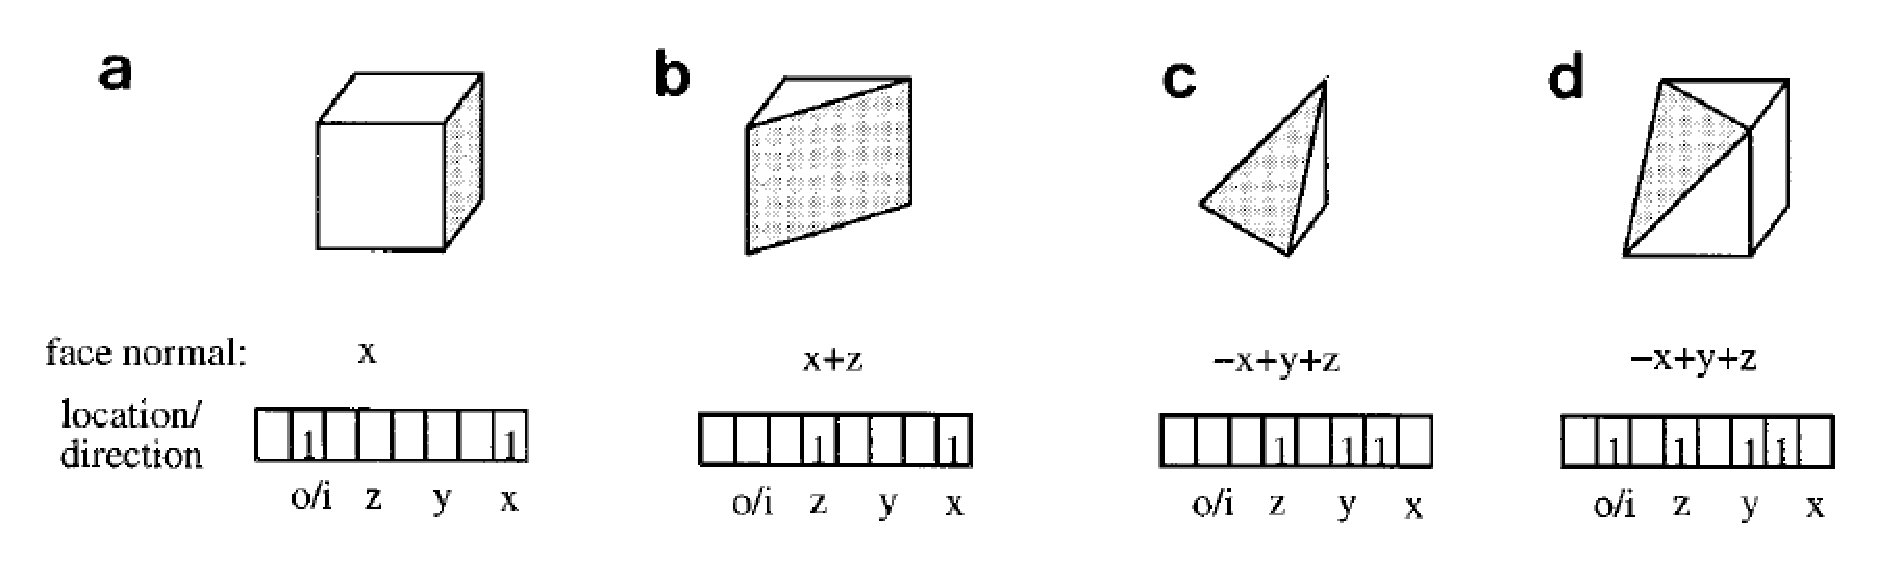
\includegraphics[height=3cm,width=10cm]{tt.eps}}
\centerline{\textbf{FIG.1.}The location/direction codes for the four volume primitives}
\begin{codebox}
  \Procname{$\proc{Surface\_Tracking}(Q\_CELL *current\_voxel)$}
  \li unsigned char index;\qquad //the table index
  \li $get\_start\_face()$;\qquad //start voxel coordinates
  \li $span\_start\_face()$;\qquad //span the start voxel
  \li \While $current\_voxel == remove\_q\_head()$
  \li \Do
  \li $x,y,z = current\_voxel->x,y,z;$
  \li $index = grad\_loc\_dir[x][y][z] \quad \& \quad \sim MARK$;
  \li $Neighbor\_face(index)$; \qquad //search for surface voxels
  \li $add\_to\_display\_table(x,y,z,index)$\qquad //add to display table
  \End
\end{codebox}


\end{document}
